\documentclass[onlytextwidth, aspectratio=169]{beamer}
\input{preamble-slides169}

%Tick mark commands
\newcommand\ticks{}
  \def\ticks{{Bar[scale=2]}-{Bar[scale=2]}}
\newcommand\paraticks{}
  \def\paraticks{{Straight Barb[reversed, scale=2]}-{Straight Barb[scale=2]}}

\title{Geometry Unit 10: Trigonometry}
\date{17 April 2023 - 5 May 2023}

\begin{document}
\frame{\titlepage}
\section[Outline]{}
\frame{\tableofcontents}

\section{10.1 Slope and the tangent function \hfill 17 April \,}
\begin{frame}{Learning Target: I can convert angle measures to slopes using the tangent function.}
  {HSG.SRT.C.8 Use trigonometric ratios and the Pythagorean Theorem to solve problems \hfill \alert{10.1 Monday 17 April}}
  \begin{columns}
    \column{0.5\textwidth}
    Do Now: Given right $\triangle$, as shown
    \begin{enumerate}
      \item What is the length of the hypotenuse?
      \item What is the slope of the hypotenuse?
      \item Estimate m$\angle A$ in degrees.
    \end{enumerate} \vspace{0.5cm}
    Lesson: The tangent function, calculator use \\[0.5cm]
    Homework: Complete the classwork practice, Deltamath problem set
    \column{0.5\textwidth}
    \begin{flushright}
      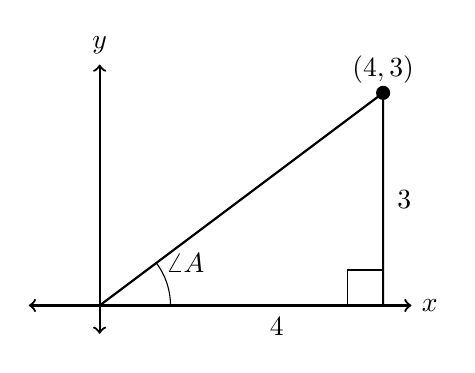
\begin{tikzpicture}[scale=0.9]
        \draw [thick, <->] (-1,0) -- (4.4,0) node [right] {$x$};
        \draw [thick, <->] (0,-0.4)--(0,3.4) node [above] {$y$};  
        \draw [thick] (0,0)--(4,0)--(4,3)--cycle;
        \draw (4,0) ++(-0.5,0)--+(0,0.5)--+(0.5,0.5);
        \node at (2.5,-0.3){4};
        %\node at (2,2.2){5};
        \node at (4.3,1.5){3};
        \fill (4,3) circle[radius=0.1] node[above] {$(4,3)$};
        \draw (1,0) arc (0:37:1)node[right] {$\angle A$};
      \end{tikzpicture}
    \end{flushright}
  \end{columns}
\end{frame}

\begin{frame}{Standard notation for trigonometric functions}
  Right triangle $\triangle ABC$ with side lengths $a$, $b$, $c$. $m\angle A = \theta$
  \begin{center}
  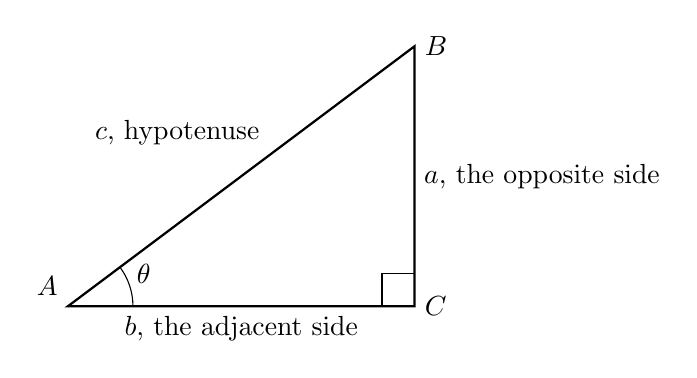
\begin{tikzpicture}[scale=0.55]
    \draw [thick](0,0)node[above left]{$A$}--
        (8,0)node[right]{$C$}--
        (8,6)node[right]{$B$}--cycle;
    \node at (1.75,0.75){$\theta$};
    \draw (1.5,0) arc (0:37:1.5);
    \draw (8,0) ++(-0.75,0)--+(0,0.75)--+(0.75,0.75);
    \node at (4,0) [below]{$b$, the adjacent side};
    \node at (8,3) [right]{$a$, the opposite side};
    \node at (0.4,4) [right]{$c$, hypotenuse};
  \end{tikzpicture}
  \end{center}
  \begin{description}
    \item[Opposite] The side across from the angle
    \item[Adjacent] The side next to the angle
    \item[Theta] A Greek letter used to represent the angle measure
    \item[tangent] The ratio of the opposite side to the adjacent side
  \end{description}
\end{frame}

\begin{frame}{Find the height of a triangle with base $b=10$ and angle 60 degrees}
  \begin{columns}
    \column{0.5\textwidth}
    \begin{center}
      $\displaystyle \tan(\theta)=\frac{opposite}{adjacent}$
      \end{center}
      Substitute the given values and use your calculator for $\tan(60^\circ)$
      \onslide<2>{\textcolor{red}{    
        \begin{center}
        $\displaystyle \tan(60^\circ)=\frac{a}{10} \approx 1.732$\\[0.5cm]
        $\displaystyle a=10\times 1.732 \approx 17.32$
        \end{center}}}
    \column{0.5\textwidth}
    \begin{flushright}
      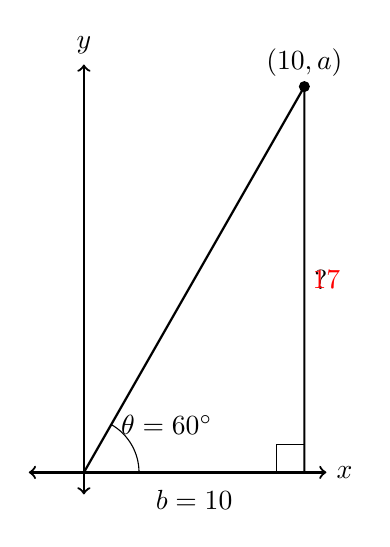
\begin{tikzpicture}[scale=0.7]
        \draw [thick, <->] (-1,0) -- (4.4,0) node [right] {$x$};
        \draw [thick, <->] (0,-0.4)--(0,7.4) node [above] {$y$};  
        \draw [thick] (0,0)--(4,0)--(4,7)--cycle;
        \draw (4,0) ++(-0.5,0)--+(0,0.5)--+(0.5,0.5);
        \node at (2,-0.5){$b=10$};
        \onslide<1>{\node at (4.3,3.5){?};}
        \onslide<2>{\node at (4.4,3.5){\textcolor{red}{17}};}
        \fill (4,7) circle[radius=0.1] node[above] {$(10,a)$};
        \draw (1,0) arc (0:60:1)node[right] {$\theta = 60^\circ$};
      \end{tikzpicture}
    \end{flushright}
  \end{columns}
\end{frame}

\section{10.2 Inverse tangent function \hfill 18 April \,}
\begin{frame}{Learning Target: I can find an angle measure using inverse tangent.}
  {CCSS.HSG.SRT.C.8 Use trig ratios and the Pythagorean Theorem to solve problems \hfill \alert{10.2 Tuesday 18 April}}
  \begin{columns}
    \column{0.6\textwidth}
    Do Now: Given right $\triangle$ shown, find its height $b$ to the \emph{nearest tenth}. \\[0.5cm]
    Lesson: The inverse tangent function, $\tan^{-1}$ \\[0.5cm]
    Homework: Complete the classwork practice, Deltamath problem set
    \column{0.4\textwidth}
    \begin{flushright}
      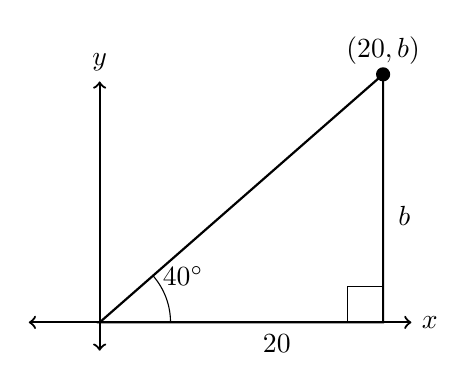
\begin{tikzpicture}[scale=0.9]
        \draw [thick, <->] (-1,0) -- (4.4,0) node [right] {$x$};
        \draw [thick, <->] (0,-0.4)--(0,3.4) node [above] {$y$};  
        \draw [thick] (0,0)--(4,0)--(4,3.5)--cycle;
        \draw (4,0) ++(-0.5,0)--+(0,0.5)--+(0.5,0.5);
        \node at (2.5,-0.3){20};
        \node at (4.3,1.5){$b$};
        \fill (4,3.5) circle[radius=0.1] node[above] {$(20,b)$};
        \draw (1,0) arc (0:41:1)node[right] {$40^\circ$};
      \end{tikzpicture}
    \end{flushright}
  \end{columns}
\end{frame}


\end{document}
